\cotefile{79}
\scanpage{160}
\mspage{81}

\uline{IX} \uline{Graphes à \deleted{opérateurs}\inserted{homothéties}.}

Nous \deleted{\unsure{prendr|prendrons}} appelons ici structure de \uline{graphes} sur un ens. de sommets $S$, la donnée d'une partie

\[ A\subset\unsure{\mathcal P|\mathfrak P}_2(S) \tag*{(1)} \]

\deleted{\unsure{N}}Nous appelerons \uline{graphe à \deleted{opérateurs}\inserted{homothéties}} une structure sur un ens. de base $S$ (l'ens de sommets) définie par la donnée de deux structures

\[ A_0\subset\mathcal P_2(S),\qquad \underset{\text{\uline{sous-groupe}}}{Z\subset\unsure{\mathfrak S|\mathscr S}_S} \tag*{(2)} \]

satisfaisant aux conditions qui suivent. Notons tout de suite qu'on ne suppose nullement que \deleted{\unsure{ceci} \uline{GH1} $Z$ est un sous-groupe de $\mathfrak S_S$} les \deleted{$\unsure{g}$} $\lambda\in Z$ respectent la structure de graphe \deleted{$\unsure{A_\lambda}$} $A$ de $S$. On suppose par contre :

\[
\begin{aligned}
 &\forall(s,t)\in S,\ \lambda\in Z,\quad \underline{\exists f}\in\mathfrak S_S,\ \text{centralisant }Z,\ \text{tel que}\\
 &\{s,t\}\in A_0\Longleftrightarrow\{f^{-1}\deleted{\unsure{\lambda|1}}s,f_{\lambda}^{-1}\deleted{\unsure{1|\lambda}}t\}\in A_0
\end{aligned}\tag*{\shortstack{(3) \deleted{\unsure{G}}\\(GH1)}}
\]

Cette condition peut se décomposer en trois

\[
\mathrm{GH1}'\left\{\begin{aligned}
\text{a)}\quad &\forall\lambda\in Z,\ \exists A_\lambda\in\mathcal P(\mathcal P_2(S))\quad\text{structure de graphe}\\
 &\text{sur }S\ \text{(évidemment unique) telle que }\forall s,t\in S\\
 &\{s,t\}\in A_0\Longleftrightarrow\{s,\lambda t\}\in A_\lambda\\
 &\text{\deleted{$[$ NB les \unsure{arêtes|étoiles} de $(S,A_0)$ et de $(S,A_\lambda)$ sont les mêmes $]$}}\\
\text{b)}\quad &\text{Cette structure de graphe $A_\lambda$ est isomorphe à $A_0$.}\\
 &\text{\deleted{\unsure{ou mieux}}}\\
 &\text{\deleted{c) Parmi les \unsure{isom.} $f\in\mathfrak S_S$ qui \unsure{établiss|centralisent} cet is}}\\
\text{c)}\quad &\text{\deleted{\unsure{isomorphisme, il en existe}} \inserted{On veut qu'il existe} un isom$^{(f)}$ de}\\
 &\text{la structure $(S,A_0,Z)$ sur la structure}\\
 &\text{$(S,A_\lambda,Z)$, et plus précisément un isom}\\
 &\text{qui \deleted{induit} \inserted{induise} l'identité sur $Z$, i.e.}\\
 &\text{par un $f\in\mathfrak S_S$ qui centralise $Z$.}
\end{aligned}\right.\tag*{(4)}
\]

% slanted
\margin{\deleted{Ceci}\inserted{a)} implique que si $\lambda,\mu\in Z$, alors $\forall s\in S$, on a $\mathrm{Et}_{A_0}((\lambda\mu)s)=\mathrm{Et}_{A_0}((\mu\lambda)s)$ donc $\lambda\mu=\mu\lambda$ si on suppose que $\begin{array}{rcl}S&\longrightarrow&\mathcal P(S)\\s&\longmapsto&\mathrm{Et}_A(s)\end{array}$ est injective. En tout état de cause, il est raisonnable de supposer $Z$ commutative.} (5) 

\deleted{On trouve} \inserted{On pose}

\[ \pi=\{A_\lambda\mid\lambda\in Z\}\subset\mathcal P(\mathcal P_2(S)) \]

\deleted{et on fait abstraction des \unsure{liens}} \inserted{et pour $i\in\pi$ on note $A_i$ au lieu de $A_\lambda$.}

% archive sheet number: 159
\scanpage{161}

On note alors que toutes les structures de graphe à homothéties $(S,A_i,Z)$, pour $i\in\deleted{\unsure{Z}}\pi$, satisfont la condition (GH1), et on a \unsure{les|en} termes de \inserted{la seule donnée} $\pi\subset\unsure{\mathcal P|\mathfrak P}(\mathcal P_2(S))$ une opération de $Z$ sur $\pi$, notée

\[
\left\{\begin{aligned}
 &\underset{\rotatebox{90}{$\in$}}{\lambda}\longmapsto\underset{\rotatebox{90}{$\in$}}{T_\lambda}
       \qquad \deleted{\unsure{\{s,t\}}}\qquad\text{définie par}\\[-2pt]
 &Z\qquad \unsure{\mathfrak S|\mathscr S}_\pi\\
 &\forall s,t\in S,\ i\in\pi,\qquad\{s,t\}\in A_i\Longleftrightarrow\{s,\lambda t\}\in A_{T_\lambda i}.
\end{aligned}\right.\tag*{\shortstack{\deleted{\unsure{(5)}}\\(6)}}
\]

\deleted{Soit \unsure{On} appelle \uline{multigraphe à opérateurs}}

Deux \deleted{$G_0=A\unsure{'|_0}$} graphes à homothéties \inserted{$(S,A_0,Z_0)(S,A_1,Z_1)$ sur le $=$ ens. de sommets} sont dits \uline{équivalents} \deleted{s'ils \unsure{=|se} peuvent se déduire l'un de l'autre par} \deleted{existe $\lambda\in Z_0$ tel que l'on ait} \deleted{$A_1=\deleted{\unsure{A}}T_\lambda(A_0)$, une opération} si on a $Z_0=Z_1$, soit $Z$, et s'il existe $\lambda\in Z$ tel qu'on ait $A_1=T_\lambda A_0$, \deleted{\unsure{donc}} ou encore si $A_1$ est $\in$ de l'ens $\pi$ construit précédemment, en termes de $(S,A_0,Z)$. Il est immédiat que c'est \inserted{bien} une \inserted{relation} \unsure{équivalence|d'équivalence}, plus restrictive que la relation d'isomorphie -- et $=$ que la relation d'isomorphie commutant à l'opération de $Z$.

La donnée, \deleted{pour} sur un ens. $S$, d'une classe d'équivalence $\pi$ en un sens de graphes à homothéties, sera appelée un \uline{multigraphe} \uline{à homothéties}. Posons alors

% archive sheet number: 160
\scanpage{162}
\mspage{82}

% slanted
\margin{autom strict d'un graphe à homoth.}

\[
G_0\ \text{ou}\ G_{A_0}=\overbrace{\operatorname{Aut}_Z(S,A_0,Z)}^{\text{autom des gr. à homothéties}}=\left\{g\in\unsure{\mathfrak S|\mathscr S}_S\,\middle|\,
\begin{array}{l}g\text{ autom. de }(S,A_0)\ \text{i.e. }g(A_0)=A_0\\g\text{ commute à }Z\end{array}\right\}\tag*{(7)}
\]

% slanted
\margin{autom strict d'un multigraphe à homoth.}

\[
\begin{aligned}
G&=\underbrace{\operatorname{Aut}_Z(S,\pi)}_{\substack{\text{autom des}\\\text{multigraphe à}\\\text{homothéties}}}
=\left\{g\in\mathfrak S_S\,\middle|\,\begin{array}{l}g\text{ autom de }(S,\pi)\ \text{i.e. }g(\pi)=\pi\\g\ \deleted{\unsure{\mathrm{se}}}\text{ commute à }Z\end{array}\right\}\\
&\hspace{1em}\text{i.e. l'opération de $g_\pi$ sur $\pi$ se fait par translation}\\
&\hspace{1em}\text{par un \unsure{él.|élt.} de $Z$}\\
&=\left\{g\in\mathfrak S_S\,\middle|\,\begin{array}{l}g\text{ commute à }Z\\g(A_0)\in\pi\end{array}\right\}
\end{aligned}\tag*{(8)}
\]

\[ G_{A_i}\quad\text{indépendant de } i\in\pi \tag*{(9)} \]

% slanted
\margin{\uline{NB} Il faudrait quand même expliciter ici des cas où la structure \unsure{a|à} $(S,\pi)$ implique déjà la \unsure{connaiss|connaissance} $\unsure{G|\text{(9)}}$, ou m$^{\rm s}$ de $Z$, et \uline{aussi} \deleted{\unsure{suffit}} des cas où tout \unsure{autom} de $(S,\pi)$ appartient déjà à \unsure{$G$|$\operatorname{Aut}G$} i.e induit l'autom. \unsure{trivial|triviale} de $Z$ (c'est le cas \unsure{ds|dans} \unsure{les situations|la situation} \unsure{congruentielles|congruentielle} particulièrement\ldots) : il suffit pour ceci que \uline{tout} autom de $(S,A_0)$ commute à $Z$ i.e soit dans $G_0$ -- ce qui est le cas dans les cas que nous avons à envisager, semble-t-il\ldots\ C'est le cas \unsure{sûrement|évidemment} dans le cas \unsure{prépolyédral régulier|des prépolyèdres réguliers} -- $\unsure{G}$ dont il sera fréquemment \unsure{question}\ldots\ Et $\bullet$ \unsure{peut} décrit $G$ en termes de $(S,F)$, ou $(S,\pi)$, on retrouve $Z$ comme le \uline{centre} de $G$. En termes d'un $(S,F_0)$ ou $(S,A_0)$ déjà donné, \deleted{\unsure{on}} mais sans s'assigner \deleted{\unsure{encore}} $\pi$, le ``meilleur choix'' d'un $Z$ qui se propose (peut-on \unsure{être} tout-à-fait valable ds le cas d'un 2-polyèdre \unsure{str$^{\rm t}$|tr.|str.} \uline{régulier}) c'est de prendre $Z=\operatorname{Comm}_{\mathfrak S_S}(G_0)$\ldots}

diagramme

\diagram{\begin{tikzcd}[ampersand replacement=\&,column sep=small,row sep=small]
(10)\quad 1\arrow[r]\&G_0\arrow[r,hook]\&G\arrow[r]\&\overset{\deleted{\unsure{Z'}}}{Z/\unsure{\mathfrak z|\zeta}}\arrow[r,dash]\&1.\\
\&\&Z\arrow[u,hook]\arrow[ur,swap,"{\lambda\mapsto\lambda^2}"]\&\&
\end{tikzcd}}

\[
\begin{aligned}
\mathfrak z&=\operatorname{Ker}(\deleted{\unsure{T}}\lambda\mapsto T_\lambda:Z\longrightarrow\mathfrak S_\pi)\\
&=\{\lambda\in Z\mid\mathrm{Et}_{A_i}(s)=\mathrm{Et}_{A_i}(\lambda s)\quad\forall s\in S,\}\ \forall i\in\pi\rbrace
\end{aligned}\tag*{(11)}
\]

\uline{NB} $\mathfrak z=\{1\}$ si tout sommet est déterminé par ses étoiles\ldots

NB Soit \deleted{\uline{NB} Soit \unsure{$A$}}

\[ \unsure{\mathcal E|\mathscr E}_{A_0}=\{E\in\unsure{\mathcal P|\mathfrak P}(S)\mid\exists s\in S;\ E=\mathrm{Et}_{A_0}(s)\} \tag*{(12)} \]

alors on a

\[ \mathcal E_{A_i}\ \text{indépendant de }i\in\pi,\quad\text{soit }\mathcal E=\mathcal E_\pi. \tag*{(13)} \]

L' \deleted{étoiles} ensemble $\mathcal E$ \inserted{$\subset\mathcal P(S)$} des étoiles pour les diverses structures de graphe $A_i$, mais le \deleted{leurs} ``centres'' \deleted{varient en \unsure{f$^{\rm t}$ d'un}} (ou les centres) d'une étoile fixée $E\subset S$ varie\unsure{(nt]|(nt)} avec la structure de graphe envisagée. Pour tt $g\in G_0$ on a $g(\mathcal E)=\mathcal E$ i.e $g$ transforme étoile en étoile. C'est le cas en particulier pour les \deleted{$\unsure{g}$} $\lambda\in Z$.

% archive sheet number: 161
\scanpage{163}

On dit qu'un graphe à homothéties est \uline{régulier} si $G_0$ (le groupe de ses autom \uline{stricts}) est transitif sur l'ens $\overrightarrow{A_0}$ de ses arêtes orientées, \inserted{et si $(S,A_0)$ n'a pas de sommet isolé et est connexe.} On dit qu'un multigraphe \deleted{est} à homothéties est régulier, si les graphes constituants le sont.

Si \deleted{$\unsure{G_0|\mathcal G}$} $(S,A_0,Z)$ est \inserted{un gr. à hom.} \uline{régulier}, $G_0$ étant transitif sur $S$, $Z$ opère \uline{librement} sur $S$. En tous cas, j'appelle \uline{\unsure{vagons|wagons|voyage}} du graphe à homothéties, \deleted{les} orbites \deleted{pour} \inserted{de} $Z$ dans $S$.

Si \inserted{on a un multigr. à hom.} \deleted{\unsure{$($}} $(S,\pi,Z)$ \deleted{est} régulier, alors \deleted{pour $i,j\in\unsure{R_\pi|\pi|\Pi}$ distincts, on a}

\[ A_i\cap A_j=\varnothing\qquad\text{si }i,j\in\pi,\quad i=j \tag*{(14)} \]

car si on a $a\in A_i\deleted{\cap A_j}$, alors $A_i$ est déterminé par $a$ comme l'orbite de $a\in\unsure{\mathcal P|\mathfrak P}_2(S)$ sous $G_0$. On trouve donc une application surjective

% slanted
\margin{La structure \inserted{de multigraphe rég.} $(S,\pi,Z)$ équivaut alors à la structure $(S,\unsure{A|F},R,Z)$, où $A\subset\mathcal P_2(S)$ muni de $Z\subset\unsure{\mathfrak S|\mathscr S}_S$, une rel. d'\unsure{équiv.|équiva.} $R$, \unsure{et où|et} (plus \unsure{ou moins|comme} bien sûr, savoir que chacun des $(S,A_i,Z)$ forme un ``graphe'' \deleted{\unsure{une}} str. de graphes à homothéties \uline{régulières}\ldots}

\[ A\overset{\mathrm{déf}}{=}\bigcup_{i\in\pi} A_i\xrightarrow{\tau_A}\pi \tag*{(15)} \]

associée à une partition

\[ A=\coprod_{i\in\pi} A_i. \tag*{(16)} \]

\deleted{Soit. On dit qu'un} \unsure{Revenant|Revenons} à un $A_0$, et posons

\[
\begin{aligned}
 F_0&=\{f\in\mathcal P_3(S)\mid\forall a\in\mathcal P_2(f),\ a\in A_0\}\\
 \text{d'où }\quad A_0&=\{a\in\mathcal P_2(S)\mid\exists f\in F_0,\ \text{\unsure{t.|,}}~ f\supset a\}.
\end{aligned}\tag*{(17)}
\]

Une structure de graphe sera dite \deleted{\unsure{prétri}} \deleted{``triangulable''} \uline{``prépolyédrale''}, si

\[ P_0=(S,A_0,F_0,\text{relations d'incidence \unsure{évidentes|évidente}}) \tag*{(18)} \]

% archive sheet number: 162
\scanpage{164}
\mspage{83}

est bel et bien un 2-polyèdre -- i.e. s'il satisfait à la condition \deleted{de connexité locale en \unsure{en} chaque sommet}

\[
\begin{aligned}
 &\forall \underset{\substack{\shortparallel\\\{s,t\}}}{a}\in A_0,\ \text{il existe exactement deux }\deleted{\unsure{f\in F_0}}\inserted{u\in S},\\
 &\text{telles que }\quad\{s,u\},\{t,u\}\in A_0,
\end{aligned}\tag*{(19)}
\]

plus la condition de connexité du contour local en tout $s\in S$. S'il en est ainsi, $G_0$ opère bien sûr par autom. de cette structure polyédrale. Si le graphe à homothéties est régulier, il \deleted{\unsure{en ré}} n'en résulte peut-être pas que le 2-polyèdre associé est régulier, \deleted{\unsure{ce}} on dit que le graphe à homothéties est \uline{str.} \uline{régulier} s'il est prépolyédral, et si $G_0$ est transitif (donc simplement transitif) sur l'ens des repères du 2-polyèdre associé.

% slanted
\margin{On a alors $F=\coprod_{i\in\pi}F_i$\ldots\ Dans le cas envisagé\unsure{,| ici,} la structure de multigraphe à hom. est défini par la connaissance de $(S,F\subset\unsure{\mathcal P|\mathfrak P}_3(S),Z\subset\unsure{\mathfrak S|\mathscr S}_S)$.}

Terminologie analogue pour les multigraphes à homothéties \uline{str.} \uline{réguliers} : Alors $G$ est simplement transitif sur l'ens. des repères de $(S,F)$.

J'ai envie de donner une description de ces derniers, en termes de théorie des groupes, en m'appuyant sur la théorie combinatoire des cartes, qui est bien comprise. Je fixe un répère \deleted{$\unsure{(s,t,u)}$ relatif à une structure \unsure{choisie ici} \unsure{constituante}}

\[ (s_0,t_0,u_0)\in\operatorname{Rep}(P_0) \tag*{(20)} \]

pour épingler la situation entièrement. \deleted{\unsure{Du coup}} On veut

% archive sheet number: 163
\scanpage{165}

tout décrire en termes de théorie des groupes, \deleted{\unsure{via une s}} \inserted{en termes} d'une structure d'extension (10). Ici on trouve des générateurs canoniques de $G_0$

\[
\left\{\begin{aligned}
 &\tau_0,\tau_1,\tau_\infty\in G_0\qquad\text{satisfaisant}\\
 &\deleted{\unsure{\tau_1|P_1}}\rho_1^{2}=\rho_\infty^3=1\qquad\text{où }\rho_1=\tau_0\tau_\infty,\ \rho_\infty=\tau_1\tau_0,\\
 &\hspace{13em}\rho_0=\tau_\infty\tau_1
\end{aligned}\right.\tag*{(21)}
\]

si $n$ est l'ordre de $\rho_0$ (il sera fini dans les cas les plus intéressants) on aura donc aussi

\[ \rho_0^n=1,\tag*{(22)} \]

$n$ sera aussi l'ordre des sommets du graphe régulier $\Gamma_0=(S,A_0)$, i.e. du 2-polyèdre régulier $P_0$. Il faut interpréter $S$ comme espace homogène sous $G$, via l'origine $s_0\in S$, donc il faut travailler avec le stabilisateur

\[ G_{s_0}=\{g\in G\mid gs_0=s_0\}=B' \tag*{\deleted{\unsure{(23)}}} \]

dont l'intersection avec $G_0$ sera donné par

\[
\begin{aligned}
B'\cap G_0&=\text{sous-groupe }\inserted{\widetilde U}\ \text{engendré}\text{ par }\tau_1,\tau_\infty\\
 &\hspace{1em}\text{(isomorphe à }\unsure{\mathbb D|D|\mathbf D}_n\text{)}
\end{aligned}\tag*{\deleted{\unsure{(24)}}}
\]

on a donc

\[
\begin{aligned}
G/B'&\stackrel{\sim}{\text{---}}S\\
g.B'&\mathrel{\unsure{\vdash\!\!-\!\dashv|\longmapsto}}g.s_0
\end{aligned}\qquad\substack{\text{isom d'espaces}\\\text{homogènes}\\\text{sous }G}\tag*{\deleted{\unsure{(25)}}}
\]

\figure{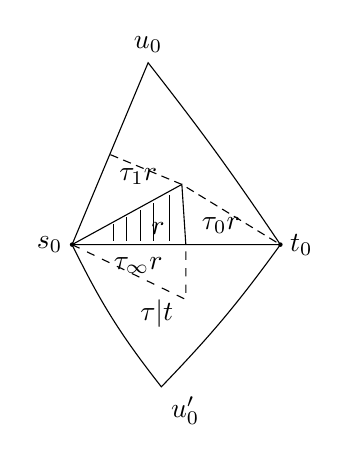
\begin{tikzpicture}[x=1cm,y=1cm,scale=.84]
\coordinate (s) at (0,0); \coordinate (t) at (3.15,0); \coordinate (u) at (1.15,2.75); \coordinate (v) at (1.35,-2.15);
\coordinate (c) at (1.66,.91); \coordinate (b) at (1.72,-.83);
\draw (s)--(u) to[bend left=2] (t)--(s) to[bend right=6] (v) to[bend right=4] (t);
\draw[densely dashed] (.58,1.36)--(c)--(t); \draw (s)--(c)--(1.72,0);
\draw[dashed] (s)--(b)--(1.72,0);
\foreach \x in {.62,.82,1.03,1.23,1.47}{\draw[thin] (\x,.06)--(\x,{.51*\x});}
\fill (s) circle (.034) (t) circle (.034);
\node[left] at (s) {$s_0$}; \node[right] at (t) {$t_0$}; \node[above] at (u) {$u_0$}; \node[below right] at (v) {$u'_0$};
\node at (1.3,.24) {$r$}; \node at (1,1.03) {$\tau_1 r$}; \node at (2.25,.29) {$\tau_0 r$}; \node at (1,-.31) {$\tau_\infty r$}; \node at (1.28,-1.05) {$\unsure{\tau|t}$};
\end{tikzpicture}}

% archive sheet number: 164
\scanpage{166}
\mspage{84}

\deleted{Notons que pour un espace homogène} Traduisons en termes de théorie des groupes, de façon tout à fait générale, la donnée suivante :

\[
\left\{\begin{aligned}
\text{a)}\quad&\text{espace homogène $S$ sous un groupe $G_0$, avec ``origine'' fixée $s_0\in S$}\\
\text{b)}\quad&\text{surgroupe $G\supset G_0$ opérant sur $S$ (en prolongeant l'action}\\
 &\text{précédente), avec $G_0$ distingué dans $G_0$ (soit $Z'=G/G_0$)}\\
\text{c)}\quad&\text{sousgroupe central $Z$ de $G$,}
\end{aligned}\right.\tag*{(26)}
\]

% slanted
\margin{\uline{NB} On ne préjuge pas, dans cette présentation, si les groupes $G_0,G$ opèrent fidèlement. On reviendra sur ce point par la suite\ldots}

en \unsure{essayant|exigeant}, dans la mesure du possible, de faire une description qui soit ``\unsure{proche|près|produite} du groupe $G_0$'', et de groupes qui se décrivent aisément en termes de $G_0$, \deleted{\unsure{de}} ses sous-groupes etc.

La donnée a) revient à la donnée du couple

\[ G_0\supset\widetilde U \tag*{(27)} \]

d'un groupe $G_0$, et d'un sous-groupe $\widetilde U$ $(=G_{0s_0})$, qui permet de \unsure{réconstruire|reconstruire} $(S,s_0)$ comme

\[ (S,s_0)\simeq(G_0/\widetilde U,\underset{\substack{\text{classe de }1_G\\\text{dans }G_0/\widetilde U}}{\dot{1}_G}). \tag*{(28)} \]

La donnée b) s'exprime, tout d'abord, comme celle d'un diagramme de groupes

\diagram{\begin{tikzcd}[ampersand replacement=\&,column sep=large]
(29)\qquad G_0\arrow[r,hook,no head, "\mathrm{dist.}"]\&G\&\\
\deleted{\unsure{G_0}}\widetilde U\arrow[u,hook,no head]\arrow[r,hook,no head]\&B'\arrow[u,hook,no head]\&(\mathrm{NB}\ B'=G_{s_0})
\end{tikzcd}}

``cartésien et cocartésien'', cartésien signifiant

\[ \widetilde U=G_0\cap B'\qquad(\text{donc }\widetilde U\text{ dist. dans }B') \tag*{(30)} \]

``cocartésien'' s'exprimant par une des deux conditions équivalentes

\[
\left\{\begin{aligned}
G_0/\widetilde U&\underset{\rm can}{\xrightarrow{\sim}}G/B' &\text{qui équivaut à}\\
B'/\widetilde U&\mathrel{\overset{\sim}{\text{---}}}G/G_0 &\text{(isom de groupes).}
\end{aligned}\right.\tag*{(31)}
\]

Le groupe $G$, extension d'un groupe

% archive sheet number: 165
\scanpage{167}

\[ Z'=G/G_0 \tag*{(32)} \]

par $G_0$, est \unsure{pour|plutôt} nous trop ``éloigné'' directement de $G_0$, on préfère l'exprimer en termes du groupe $B'$, extension d'un même $Z'$ par \deleted{le} \inserted{un} groupe $\deleted{\unsure{B|M}}\widetilde U$ de $G$ (en pratique, $Z'\simeq(\mathbb Z/n\mathbb Z)^*$ ou $(\mathbb Z/n\mathbb Z)^*/\pm1$, $\widetilde U\simeq\mathbb Z/n\mathbb Z$ ou $\unsure{\mathbb D|D|\mathbf D}_n$, sont deux groupes bien compris et ``petits'', leur extension sera aussi bien \unsure{pigeable|pignable|pignolle|gérable}).

En vertu des \unsure{topoïs|topis|topos|tapis} bien connus, pour reconstituer l'extension $G$ de $Z'$ par $G_0$ à l'aide de l'extension $B'$ de $Z'$ par $\widetilde U$, par une sorte de \deleted{chgt. de} \inserted{extension} du groupe noyau $\widetilde U\hookrightarrow G_0$, il faut de plus se donner l'opération

\[ B'\mathrel{\longrightarrow}\operatorname{Aut}_{\rm gr}(G_0) \tag*{(33)} \]

prolongeant l'opération tautologique du sous-groupe $\widetilde U$ de $B'$ sur $G_0\supset\widetilde U$, par autom intérieurs.

Ainsi, les données (a) (b) de (26) équivalent aux données

\[
\left\{\begin{aligned}
\text{a)}\quad&\text{une extension \inserted{$B'$} d'un groupe $Z'$ par un groupe $\widetilde U$}\\
 &1\mathrel{\text{---}}\deleted{\unsure{B}}\widetilde U\mathrel{\text{---}}B'\mathrel{\text{---}}Z'\mathrel{\unsure{\text{---}|\longrightarrow}}1\\
\text{b)}\quad&\text{un hom. injectif de groupes}\\
 &\widetilde U\hookrightarrow G_0\\
\text{c)}\quad&\text{une opération (33) de $B'$ sur $G_0$, prolongeant}\\
 &\text{l'opération de $\widetilde U$ déduite de b).}
\end{aligned}\right.\tag*{(34)}
\]

Pour interpréter la donnée c) de (26), on commence à noter \deleted{que le \unsure{commutant}} \inserted{l'isomorphisme} de groupes

% archive sheet number: 166
\scanpage{168}
\mspage{85}

\[ \substack{\text{Commutant}\\\text{de }G_0\text{ dans }\unsure{\mathfrak S|\mathscr S}_S}\simeq\operatorname{Norm}_{G_0}(\widetilde U)/\widetilde U \tag*{(35)} \]

donc la donnée d'un sous-groupe $Z$ du commutant revient à la donnée d'un sous-groupe $\widetilde B''$ de $G_0$, \deleted{\unsure{en}} satisfaisant

\[ \widetilde U\subset\widetilde B''\subset\operatorname{Norm}_{G_0}(\widetilde U),\quad\text{avec }Z= \tag*{(36)} \]

\inserted{i.e. $\widetilde B''$ un sous-groupe de $G_0$, contenant $\widetilde U$ comme sous-groupe \uline{distingué} de sorte qu'on a un groupe quotient $Z=\widetilde B''/\widetilde U$}

en termes de (26) on aura

\[ \widetilde B''=\{g\in G_0\mid gs_0\in Z.s_0\}.\tag*{(37)} \]

La condition que $Z$ commute non seulement à l'action de $G_0$, mais aussi à l'action de $G$ \deleted{tout} entier, ou ce qui revient au $=$ de $B'$ (puisque $G=B'.G_0$ \} produit de sous-ens. de $G$) s'explicite aisément par \inserted{l'une} des conditions équivalentes

\[
\begin{aligned}
\text{a)}\quad&\widetilde B''\text{ normalise le sous groupe $B'$ de $G$, ou encore :}\\
\text{b)}\quad&B'\text{ normalise $\widetilde B''$ (pour l'action (33)) et l'action}\\
&\text{dans le quotient $\widetilde B''/\widetilde U$ est triviale.}
\end{aligned}\tag*{(38)}
\]

Ici c'est bien sûr la forme 38 b) qui sera la plus maniable pour notre propos, \deleted{\unsure{en|$Z$}} s'exprimant directement en termes des données (39) et (36). Nous pouvons introduire alors le \inserted{ss-}groupe $B$ de $G$ engendré par $\widetilde B'',B'$, qui s'insère dans le diagramme

\diagram{\begin{tikzcd}[ampersand replacement=\&,column sep=normal,row sep=small]
(39)\quad\&G_0\arrow[r,dash,"Z'"]\arrow[d,dash]\&G\arrow[d,dash]\\
\&\widetilde B''\arrow[r,dash,"Z'"]\arrow[d,dash,"Z"']\&B\arrow[d,dash,"Z"]\\
\&\widetilde U\arrow[r,dash,"Z'"]\&B'
\end{tikzcd}}

où on a marqué au dessus des flèches d'\unsure{inclusions|inclusion}, d'un

% archive sheet number: 167
\scanpage{169}

sous-groupe distingué ds un groupe ambiant, la valeur du groupe quotient. Les deux carrés de ce diagramme sont cartésiens et cocartésiens -- en particulier, $B$ avec son sous-groupe invariant \deleted{\unsure{$g$}} $\widetilde B''$, se déduit de $(B'\supset\widetilde U)$ et de l'action de $B'$ sur $\widetilde B''$ (induite par (33)), de la $=$ façon que $(G\supset G_0)$ se déduit de $(B'\supset\widetilde U)$ et de l'action (33) de $B'$ sur $G_0$.

Le groupe $\widetilde B''$ \deleted{\unsure{est, ici}} sera, dans les cas qui nous occupent, ``petits'' et bien \unsure{pigeables|pignables|figurables} \inserted{(en plus d'être plongé dans $G_0$)}, au $=$ titre que $B'$ auquel il ressemble comme un frère, et il en sera de $=$ de $B$.

Nous avons exprimé pour l'instant \inserted{dans (26 c))} la donnée d'un sous-groupe $Z$ de $\unsure{\mathfrak S|\mathscr S}_S$ commutant à l'action de $G$, mais il reste encore à exprimer que $Z$ est donné en \deleted{tant} que sous-groupe central de $G$. Cela s'explicite par la donnée d'un homomorphisme \deleted{$\unsure{Z}$}

\[ Z\longrightarrow G \tag*{(40)} \]

tel que les deux actions de $Z$ sur $S$ -- celles du début, et celle déduite de (40), soient égales.

On voit alors tout de suite que cela signifie que \deleted{l'on a} \inserted{(40) provient} d'un \uline{scindage} \deleted{\unsure{central}} \inserted{``central''} de l'extension $B$ de $Z$ par $B'$, \deleted{qui est}

\diagram{\begin{tikzcd}[ampersand replacement=\&,column sep=small,row sep=tiny]
(41)\quad\left\{\vphantom{\begin{matrix}X\\X\\X\end{matrix}}\right.\ 0\arrow[r,dash]\&B'\arrow[r]\&B\arrow[r,dash]\&Z\arrow[r,dash]\arrow[l,bend left=38]\&0
\end{tikzcd}}

définissant \inserted{donc} un isomorphisme $B\simeq\deleted{\unsure{B'}}Z\times B'$ avec en plus $Z$\inserted{$\subset\unsure{B|B'}$} opérant \uline{trivialement} sur $G_0$ (donc sur $G$)

% archive sheet number: 168
\scanpage{170}
\mspage{86}

Nous allons reformuler les données (\unsure{39|34})(36) et (41) (le scindage \deleted{\unsure{$g$|$\xi$}} de l'extension $B$ de $Z$ par $B'$) en \deleted{\unsure{inter}}\inserted{les} réinterprétant \deleted{ce diagramme comme \unsure{donnée}} \inserted{comme l'une des} \deleted{\unsure{don}}nées suivantes

\noindent\begin{tabular}{@{}l@{}l@{}}
(42)\ $\left\{\vphantom{\rule{0pt}{11cm}}\right.$ & \begin{minipage}{.84\linewidth}
a) Un diagramme \inserted{carré} de groupes, cartésien et cocartésien, avec des inclusions de groupes qui sont \unsure{distingués|distingué}

\diagram{\begin{tikzcd}[ampersand replacement=\&,row sep=small]
\widetilde B''\arrow[r,hook,"Z'"]\&B\\
\widetilde U\arrow[u,hook,no head,"Z"]\arrow[r,hook,"Z'"]\&B'\arrow[u,hook,"Z"']
\end{tikzcd}}

b) Un scindage de l'extension $B$ de $Z$ par $B'$, avec un groupe-section $Z\subset B$ central dans $B$, de sorte que l'on a un iso. d'ext.

\[ B\simeq B'\times Z,\qquad \deleted{\unsure{B}}Z\simeq\widetilde B''/\widetilde U\ \text{commutatif} \]

c) Un \deleted{opération de} \inserted{plongement} de groupes

\[ \widetilde B''\mathrel{\unsure{\lhook\joinrel-|\hookrightarrow}}G_0 \]

d) Une opération de $B$ sur $G_0$,

\[ B\longrightarrow\operatorname{Aut}_{\rm gr}(G_0) \]

prolongeant l'opération tautologique de $\widetilde B''$ sur $G_0$ déduite de c), et \uline{triviale} sur le sous-groupe $Z$ de $B$. (opération qui permet alors de réconstituer le groupe $G$ et le diagramme (39))
\end{minipage}\end{tabular}

Nous allons encore modifier un peu cette traduction, en écrivant le diagramme (42 a) \inserted{$+$ donnée b)} sous la forme

\diagram{\begin{tikzcd}[ampersand replacement=\&,row sep=small]
(43)\quad\&\widetilde B''\arrow[r,hook,"{\deleted{\unsure{Z'}}}","{\unsure{i|t}}"']\&B'\times Z\&\\
\&\widetilde U\arrow[u,hook,"Z"]\arrow[r,hook,"Z'"]\&B'=B'\times\{0\}\arrow[u,hook]\& Z=\widetilde B''/\widetilde U
\end{tikzcd}}

% archive sheet number: 169
\scanpage{171}
\mspage{87}

\unsure{qui|Qui} se réconstitue à partir du diagramme de groupes partiel

\diagram{\begin{tikzcd}[ampersand replacement=\&,row sep=small]
(44)\quad\&\widetilde B''\&\\
\&\widetilde U\arrow[u,hook,"Z"]\arrow[r,hook,"Z'"]\&B'
\end{tikzcd}}

sauf que pour en tirer l'hom horizontal $i$ de (43), dont la composante suivant $Z$ doit être l'hom can de passage au quotient, il faut se donner la première composante, savoir un homomorphisme de groupes

\[ \widetilde B''\longrightarrow B' \]

la commutativité de (43) signifiant que ce dernier rend commutatif le triangle

\diagram{\begin{tikzcd}[ampersand replacement=\&,row sep=small]
(45)\quad\&\widetilde B''\arrow[dr]\&\\
\&\widetilde U\arrow[u,hook,"Z"]\arrow[r,hook,"Z'"]\&B'
\end{tikzcd}}

de telle sorte qu'elle donne \inserted{donc} naissance à un hom. d'extensions de groupes

\diagram{\begin{tikzcd}[ampersand replacement=\&,column sep=small,row sep=small]
(\unsure{45|46})\quad 1\arrow[r,dash]\&\widetilde U\arrow[r]\arrow[d,"1"]\&\widetilde B''\arrow[r]\arrow[d,"\psi"]\&Z\arrow[r,dash]\arrow[d]\&1\\
1\arrow[r,dash]\&\widetilde U\arrow[r]\&B'\arrow[r]\&Z'\arrow[r,dash]\&1.
\end{tikzcd}}

Ainsi, les données (42 a)b)) se réduisent à la donnée d'un hom de suites exactes (46), ou encore d'un diagramme d'hom de groupes

\diagram{\begin{tikzcd}[ampersand replacement=\&,row sep=tiny]
(47)\quad\&\&Z\arrow[d]\\
\&B'\arrow[r,"\text{épi}"']\&Z',
\end{tikzcd}}

% archive sheet number: 170
\scanpage{172}
\mspage{88}

dont on \deleted{\unsure{dé}}déduit $\widetilde U$ \deleted{comme $\operatorname{Ker}(B'\longrightarrow Z')$}, et $\widetilde B''$ comme .

\[
 \underbrace{\widetilde B''\simeq B'\times_{Z'}Z}_{\substack{\text{image inv. de}\\\text{l'ext $B'$ de $Z'$ par $\widetilde U$,}\\\text{par l'hom }Z\mathrel{\text{---}} Z'}},
 \qquad\widetilde U=\operatorname{Ker}(B'\mathrel{\unsure{\text{---}\bullet|\longrightarrow}} Z').\tag*{(48)}
\]

\deleted{Ceci dit,} \inserted{Il me semble} que c'est sous la forme (46), où $\widetilde B''$ figure déjà nommément, que la donnée est \inserted{cependant} la plus maniable, puisque c'est \deleted{\unsure{sur|sous}} $\widetilde B''$ qui intervient directement dans la donnée (42\deleted{\unsure{b}} c).

\deleted{\unsure{Il}} Pour expliciter enfin la donnée (42 d), en écrivant $B=B'\times Z$, et en notant que l'opération de $B$ sur $G_0$ doit être triviale sur $Z$, on voit que cette donnée se réduit à celle d'une op. de $B'$ sur $G_0$ ; \deleted{\unsure{i.e.} (33)} pour écrire que \deleted{cette} l'opération \inserted{de $B$ sur $\unsure{G|G_0}$} se réduit sur $\widetilde B''$ à l'opération tautologique déduite du plongement $\widetilde B''\subset G_0$, on note que l'opération en question sur $\widetilde B''$ est l'opération composée

\[ \widetilde B''\longrightarrow B'\longrightarrow\operatorname{Aut}_{\rm gr}(G_0) \tag*{(49)} \]

qui doit donc être l'opération tautologique.

En résumé, on trouve que les données (26) s'explicitent en termes de théorie des

% archive sheet number: 171
\scanpage{173}

groupes par les données suivantes

\[
\left\{\begin{aligned}
\text{a)}\quad&\text{Un diagramme de groupes}\\
 &\widetilde U\subset\widetilde B''\subset G_0,\quad\text{avec $\widetilde U$ distingué dans $\widetilde B''$}\\
 &\deleted{\unsure{b)}}\quad\text{d'où un groupe quotient}\\
 &Z=\widetilde B''/\widetilde U\qquad(\widetilde B''\text{ ext. de $Z$ par $\widetilde U$})\\
\text{b)}\quad&\text{Un \deleted{hom.} hom de groupes }Z\xrightarrow{\unsure{\epsilon|\varepsilon}}Z'\quad\text{et}\\
 &\text{une extension \inserted{$B'$} de $Z'$ par le $\widetilde U$ du a,}\\
 &\text{de telle façon que $\widetilde B''$ soit déduit de}\\
 &\text{cette extension par l'hom $Z\mathrel{\text{---}}Z'$, i.e.}\\
 &\text{qu'on ait un hom de suites exactes (46)}\\
\text{c)}\quad&\text{Une opération de $B'$ sur $G_0$, de telle}\\
 &\text{façon que l'opération composée}\\
 &\widetilde B''\xrightarrow{\psi}B'\mathrel{\text{---}}\operatorname{Aut}_{\rm gr}(G_0)\\
 &\text{soit l'opération tautologique déduite du}\\
 &\text{plongement a) de $\widetilde B''$ dans $G_0$.}
\end{aligned}\right.\tag*{(50)}
\]

% slanted
\margin{oublié : la condition que pour $g\in\widetilde B^{\unsure{\prime\prime|\prime}}$, $\Theta(g)|U=\operatorname{int}(g)|U$, et que $\unsure{\Theta g)|\Theta(g)|\theta(g)}$ normalise $U$ et centralise $\widetilde B''$ mod $U$}

En termes des données (26), on a

\[
\left\{\begin{aligned}
 &\deleted{\unsure{B}}\widetilde U=G_{0s_0}\underset{\unsure{\mathrm{df}|\times}}{=}\deleted{\unsure{B}}\{g\in G_0\mid g.s_0=s_0\}\\
 &\widetilde B''=\{g\in G_0\mid gs_0\in Z.s\}\\
 &Z'=G/G_0,\quad Z\longrightarrow Z'\quad\text{le composé }Z\underset{\rm incl.}{\subset}G\xrightarrow{\rm can}\underbrace{G/G_0}_{Z'}\\
 &B'=\deleted{\unsure{\{g\in}}G_{s_0}=\{g\in G\mid gs_0=s_0\}\quad\text{de sorte que}\\
 &\deleted{\unsure{\widetilde U=B'|Z=}}\quad\widetilde U=B'\cap G_0,\quad B'\longrightarrow Z'\ \text{composé }B'\underset{\rm incl}{\subset}G\xrightarrow{\rm can}\underbrace{G/G_0}_{Z'}\\
 &\text{Op. de $B'$ sur $G_0$ induite par celle de $G$ sur}\\
 &\text{le sous-groupe distingué $G_0$}
\end{aligned}\right.\tag*{(51)}
\]

En termes des données (\unsure{50|80}), on récupère (26) par

\[
\left\{\begin{aligned}
\text{a)}\quad&G\ \text{ext. de $Z'$ par $G_0$ déduite de \deleted{$\unsure{B'}$} l'ext \inserted{b)} $B'$ de $Z'$ par $\widetilde U$,}\\
 &\text{le plongement $\widetilde U\mathrel{\lhook\joinrel-}G_0$, et l'opération \inserted{c)} de $B'$ sur $G_0$.}\\
\text{b)}\quad&S\simeq G_0/\widetilde U\simeq G/B'\\
\text{c)}\quad&Z=\operatorname{Im}(\widetilde B''\xrightarrow{\unsure{\varphi|\phi}}G),\quad\varphi(g)=g.\psi(g)^{-1}\\
 &\hspace{16em}=\psi(g)^{-1}.g
\end{aligned}\right.\tag*{(52)}
\]

\margin{produit dans $G$ qui contient $\widetilde B'',B'$, $\psi:\widetilde B''\mathrel{\text{---}}B'$ défini dans (50 c).}

\margin{\uline{NB} L'hom $\varphi:\widetilde B''\longrightarrow G$ se factorise par \unsure{le|son} quotient $\widetilde B''/\widetilde U\simeq Z$}

% archive sheet number: 172
\scanpage{174}
\mspage{89}

\uline{NB} On a un hom unique (\unsure{via|vu|où|sous} les données (50))

\[\unsure{\varphi|\phi}_Z:\ Z=\widetilde B''/\widetilde U\longrightarrow G\tag*{(53)}\]

\deleted{\unsure{défini p.|défini}} défini par factorisation à partir de l'application

\[\begin{aligned}\varphi=\varphi_{\widetilde B''}:\quad&\widetilde B''\mathbin{\unsure{\text{---}\bullet|\longrightarrow}}G\\
&\varphi(g)=g\psi(g)^{-1}=\psi(g)^{-1}g
\end{aligned}\tag*{(54)}\]

où l'égalité des deux expressions provient de la relation

\[\psi(g)\deleted{\unsure{p|b}}h\psi(g)^{-1}=ghg^{-1}\qquad\text{pour }\begin{gathered}g\in\widetilde B''\\h\in G_0\end{gathered}\tag*{(55)}\]

(cf (50 c)). La chose essentielle à vérifier est la multiplicativité de $\varphi$ définie par (54), étant évident qu'elle est triviale sur $\widetilde U$ puisque pour $g\in\widetilde U)$ on a $\psi(g)=g$ d'où $\varphi(g)=1$. \deleted{\unsure{Pour un|Comme}} Il faut vérifier

\[\begin{aligned}
\deleted{\unsure{g}}\quad g\psi(g)^{-1}\underbrace{g'\psi(g')^{-1}}_{\text{commutent}}&\overset{?}{=}gg'\psi(gg')^{-1}\qquad g,g'\in B'\\
\text{i.e.}\qquad \underbrace{\psi(g)^{-1}\psi(g')^{-1}}_{\psi(g'g)^{-1}}&\overset{?}{=}g'\psi(gg')^{-1}g'^{-1}
\end{aligned}\]

Comme $Z=\widetilde B''/\widetilde U$ est commutatif, on aura

\[g'g=gg'u\quad\deleted{d'où}\ (\text{i.e }u=g'^{-1}g^{-1}g'g\ \text{soit }u^{-1}=g^{-1}g'^{-1}gg')\]

\[\psi(g'g)^{-1}=\psi(gg'u)^{-1}=\psi(u^{-1})^{\deleted{\unsure{-1}}}\psi(gg')^{-1},\quad\text{et la}\]

relation à vérifier s'écrit

\[\underset{\substack{\Vert\\u^{-1}=g^{-1}g'^{-1}gg'}}{\psi(u^{-1})}\ \overset{?}{=}\ g'\underbrace{\psi(gg')^{-1}g'^{-1}\psi(gg')}_{(gg')^{-1}g'^{-1}(gg')\quad(55)}\]

soit

\[g^{-1}g'^{-1}gg'=g'g'^{-1}g^{-1}g'^{-1}gg'\qquad\text{ok}.\]

% archive sheet number: 173
